% Part 5: Two-Layer Agent Architecture
% Beamer Presentation with UofSC Branding
\documentclass[aspectratio=169,11pt]{beamer}

% ============================================================
% PACKAGES
% ============================================================
\usepackage[utf8]{inputenc}
\usepackage[T1]{fontenc}
\usepackage{lmodern}
\usepackage{tikz}
\usetikzlibrary{shapes.geometric, arrows.meta, positioning, fit, calc, backgrounds}
\usepackage{listings}
\usepackage{xcolor}
\usepackage{booktabs}
\usepackage{array}
\usepackage{multirow}
\usepackage{graphicx}
\usepackage{fontawesome5}

% ============================================================
% UofSC COLOR DEFINITIONS
% ============================================================
% Primary Colors
\definecolor{UofSCGarnet}{HTML}{73000a}
\definecolor{UofSCBlack}{HTML}{000000}
\definecolor{UofSCWhite}{HTML}{ffffff}

% Accent Colors
\definecolor{UofSCRose}{HTML}{CC2E40}
\definecolor{UofSCAtlantic}{HTML}{466A9F}
\definecolor{UofSCCongaree}{HTML}{1F414D}
\definecolor{UofSCHorseshoe}{HTML}{65780B}
\definecolor{UofSCGrass}{HTML}{CED318}
\definecolor{UofSCHoneycomb}{HTML}{A49137}

% Neutral Colors
\definecolor{UofSC90Black}{HTML}{363636}
\definecolor{UofSC70Black}{HTML}{5C5C5C}
\definecolor{UofSC50Black}{HTML}{A2A2A2}
\definecolor{UofSCWarmGrey}{HTML}{676156}
\definecolor{UofSCSandstorm}{HTML}{FFF2E3}

% Special Colors
\definecolor{UofSCDarkGarnet}{HTML}{570008}
\definecolor{UofSCAzalea}{HTML}{844247}

% ============================================================
% BEAMER THEME CONFIGURATION
% ============================================================
\usetheme{Madrid}
\usecolortheme{default}

% Override colors with UofSC palette
\setbeamercolor{palette primary}{bg=UofSCGarnet,fg=UofSCWhite}
\setbeamercolor{palette secondary}{bg=UofSCCongaree,fg=UofSCWhite}
\setbeamercolor{palette tertiary}{bg=UofSCAtlantic,fg=UofSCWhite}
\setbeamercolor{palette quaternary}{bg=UofSCBlack,fg=UofSCWhite}

\setbeamercolor{structure}{fg=UofSCGarnet}
\setbeamercolor{section in toc}{fg=UofSCBlack}
\setbeamercolor{subsection in toc}{fg=UofSC70Black}

\setbeamercolor{title}{fg=UofSCWhite,bg=UofSCGarnet}
\setbeamercolor{frametitle}{fg=UofSCWhite,bg=UofSCGarnet}
\setbeamercolor{framesubtitle}{fg=UofSCWhite}

\setbeamercolor{block title}{bg=UofSCGarnet,fg=UofSCWhite}
\setbeamercolor{block body}{bg=UofSCSandstorm,fg=UofSCBlack}
\setbeamercolor{block title alerted}{bg=UofSCRose,fg=UofSCWhite}
\setbeamercolor{block body alerted}{bg=UofSCSandstorm,fg=UofSCBlack}
\setbeamercolor{block title example}{bg=UofSCAtlantic,fg=UofSCWhite}
\setbeamercolor{block body example}{bg=UofSCSandstorm,fg=UofSCBlack}

\setbeamercolor{item}{fg=UofSCGarnet}
\setbeamercolor{subitem}{fg=UofSCAtlantic}
\setbeamercolor{subsubitem}{fg=UofSCCongaree}

\setbeamercolor{description item}{fg=UofSCGarnet}
\setbeamercolor{caption name}{fg=UofSCGarnet}

\setbeamercolor{footnote}{fg=UofSC70Black}
\setbeamercolor{footnote mark}{fg=UofSCGarnet}

% Remove rounded corners - sharp edges only
\setbeamertemplate{blocks}[default]
\setbeamertemplate{title page}[default][colsep=-4bp,rounded=false,shadow=false]
\setbeamertemplate{frametitle}[default][colsep=-4bp,rounded=false,shadow=false]

% Navigation symbols
\setbeamertemplate{navigation symbols}{}

% Itemize/enumerate settings
\setbeamertemplate{itemize items}[square]
\setbeamertemplate{enumerate items}[default]

% ============================================================
% LISTINGS CONFIGURATION
% ============================================================
\lstset{
    basicstyle=\ttfamily\scriptsize,
    keywordstyle=\color{UofSCGarnet}\bfseries,
    commentstyle=\color{UofSC70Black}\itshape,
    stringstyle=\color{UofSCAtlantic},
    backgroundcolor=\color{UofSCSandstorm},
    frame=single,
    framerule=0.5pt,
    rulecolor=\color{UofSC50Black},
    showstringspaces=false,
    breaklines=true,
    breakatwhitespace=true,
    tabsize=2,
    xleftmargin=3pt,
    xrightmargin=3pt,
    aboveskip=5pt,
    belowskip=5pt
}

\lstdefinelanguage{pseudo}{
    morekeywords={task, if, else, for, while, return, spawn, wait, collect, synthesize},
    sensitive=true,
    morecomment=[l]{//},
    morecomment=[s]{/*}{*/},
    morestring=[b]",
}

% ============================================================
% TIKZ STYLES
% ============================================================
\tikzset{
    % Box styles - all sharp corners
    orchestrator/.style={
        rectangle,
        draw=UofSCGarnet,
        fill=UofSCGarnet!10,
        line width=1.5pt,
        minimum width=4cm,
        minimum height=1.2cm,
        align=center,
        font=\bfseries
    },
    worker/.style={
        rectangle,
        draw=UofSCAtlantic,
        fill=UofSCAtlantic!10,
        line width=1pt,
        minimum width=2cm,
        minimum height=0.9cm,
        align=center
    },
    task/.style={
        rectangle,
        draw=UofSCCongaree,
        fill=UofSCCongaree!10,
        line width=1pt,
        minimum width=1.8cm,
        minimum height=0.8cm,
        align=center
    },
    process/.style={
        rectangle,
        draw=UofSCBlack,
        fill=UofSCWhite,
        line width=1pt,
        minimum width=3cm,
        minimum height=0.8cm,
        align=center
    },
    result/.style={
        rectangle,
        draw=UofSCHorseshoe,
        fill=UofSCHorseshoe!10,
        line width=1pt,
        minimum width=2.5cm,
        minimum height=0.8cm,
        align=center
    },
    decision/.style={
        diamond,
        draw=UofSCGarnet,
        fill=UofSCGarnet!10,
        line width=1pt,
        minimum width=2cm,
        minimum height=1cm,
        align=center,
        aspect=2
    },
    % Arrow styles - straight lines only
    arrow/.style={
        ->,
        >=Stealth,
        line width=1pt,
        draw=UofSCBlack
    },
    thickarrow/.style={
        ->,
        >=Stealth,
        line width=1.5pt,
        draw=UofSCGarnet
    },
    dashedarrow/.style={
        ->,
        >=Stealth,
        line width=1pt,
        draw=UofSC70Black,
        dashed
    }
}

% ============================================================
% DOCUMENT INFO
% ============================================================
\title[Two-Layer Agent Architecture]{Two-Layer Agent Architecture}
\subtitle{Orchestration and Specialization in Agentic Coding}
\author{Teaching Agentic Coding Tools}
\institute{University of South Carolina}
\date{\today}

% ============================================================
% DOCUMENT BEGIN
% ============================================================
\begin{document}

% ------------------------------------------------------------
% TITLE SLIDE
% ------------------------------------------------------------
\begin{frame}[plain]
\titlepage
\end{frame}

% ------------------------------------------------------------
% TABLE OF CONTENTS
% ------------------------------------------------------------
\begin{frame}{Outline}
\tableofcontents
\end{frame}

% ============================================================
% SECTION 1: Introduction to Two-Layer Pattern
% ============================================================
\section{Introduction to Two-Layer Pattern}

% ------------------------------------------------------------
% Slide 1: Title - Architecture Overview
% ------------------------------------------------------------
\begin{frame}{Two-Layer Agent Architecture: Overview}
\begin{columns}[T]
\begin{column}{0.55\textwidth}
\begin{center}
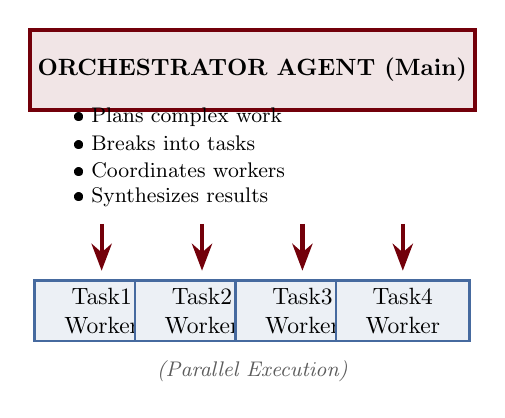
\begin{tikzpicture}[scale=0.85, transform shape]
    % Orchestrator
    \node[orchestrator, minimum width=6cm] (orch) at (0,3) {ORCHESTRATOR AGENT (Main)};

    % Orchestrator responsibilities
    \node[anchor=west, font=\small] at (-2.8,2.3) {\textbullet\ Plans complex work};
    \node[anchor=west, font=\small] at (-2.8,1.9) {\textbullet\ Breaks into tasks};
    \node[anchor=west, font=\small] at (-2.8,1.5) {\textbullet\ Coordinates workers};
    \node[anchor=west, font=\small] at (-2.8,1.1) {\textbullet\ Synthesizes results};

    % Arrows down
    \foreach \x in {-2.25,-0.75,0.75,2.25} {
        \draw[thickarrow] (\x,0.7) -- (\x,0);
    }

    % Workers
    \node[worker] (w1) at (-2.25,-0.6) {Task1\\Worker};
    \node[worker] (w2) at (-0.75,-0.6) {Task2\\Worker};
    \node[worker] (w3) at (0.75,-0.6) {Task3\\Worker};
    \node[worker] (w4) at (2.25,-0.6) {Task4\\Worker};

    % Parallel label
    \node[font=\small\itshape, text=UofSC70Black] at (0,-1.5) {(Parallel Execution)};
\end{tikzpicture}
\end{center}
\end{column}
\begin{column}{0.45\textwidth}
\begin{block}{Key Concepts}
\begin{itemize}
    \item Modern agentic coding uses two layers
    \item \textbf{Orchestrator:} Strategic planning
    \item \textbf{Workers:} Focused execution
    \item Enables scaling and parallelization
    \item Mirrors human project management
\end{itemize}
\end{block}
\vspace{0.3cm}
\textbf{Key Insight:} Separation of concerns through orchestration-worker division
\end{column}
\end{columns}

\note{The two-layer pattern is fundamental to effective agentic coding at scale. Instead of one agent trying to do everything, we separate concerns: one agent orchestrates and plans, while specialized workers execute discrete tasks.}
\end{frame}

% ------------------------------------------------------------
% Slide 2: What is Orchestration?
% ------------------------------------------------------------
\begin{frame}{Orchestration: The Art of Coordinating Agents}
\begin{columns}[T]
\begin{column}{0.5\textwidth}
\begin{center}
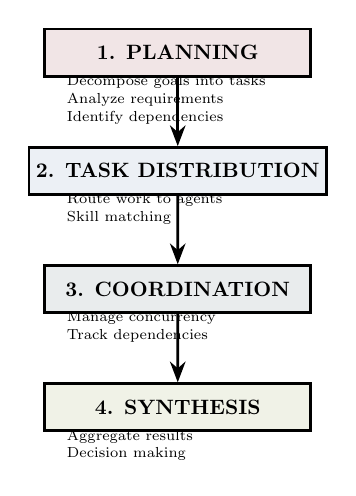
\begin{tikzpicture}[scale=0.75, transform shape]
    % Planning box
    \node[process, minimum width=4.5cm, fill=UofSCGarnet!10] (plan) at (0,4) {\textbf{1. PLANNING}};
    \node[anchor=west, font=\scriptsize] at (-2,3.5) {Decompose goals into tasks};
    \node[anchor=west, font=\scriptsize] at (-2,3.2) {Analyze requirements};
    \node[anchor=west, font=\scriptsize] at (-2,2.9) {Identify dependencies};

    % Distribution box
    \node[process, minimum width=4.5cm, fill=UofSCAtlantic!10] (dist) at (0,2) {\textbf{2. TASK DISTRIBUTION}};
    \node[anchor=west, font=\scriptsize] at (-2,1.5) {Route work to agents};
    \node[anchor=west, font=\scriptsize] at (-2,1.2) {Skill matching};

    % Coordination box
    \node[process, minimum width=4.5cm, fill=UofSCCongaree!10] (coord) at (0,0) {\textbf{3. COORDINATION}};
    \node[anchor=west, font=\scriptsize] at (-2,-0.5) {Manage concurrency};
    \node[anchor=west, font=\scriptsize] at (-2,-0.8) {Track dependencies};

    % Synthesis box
    \node[process, minimum width=4.5cm, fill=UofSCHorseshoe!10] (synth) at (0,-2) {\textbf{4. SYNTHESIS}};
    \node[anchor=west, font=\scriptsize] at (-2,-2.5) {Aggregate results};
    \node[anchor=west, font=\scriptsize] at (-2,-2.8) {Decision making};

    % Arrows
    \draw[arrow] (plan) -- (dist);
    \draw[arrow] (dist) -- (coord);
    \draw[arrow] (coord) -- (synth);
\end{tikzpicture}
\end{center}
\end{column}
\begin{column}{0.5\textwidth}
\begin{block}{Orchestrator Responsibilities}
\begin{itemize}
    \item Coordination layer managing multiple agents
    \item Decides \textbf{WHAT} work and \textbf{WHO} does it
    \item Does not execute work directly
\end{itemize}
\end{block}

\begin{alertblock}{Requires Understanding}
\begin{itemize}
    \item Problem decomposition
    \item Agent capabilities
    \item Dependency management
    \item Result integration
\end{itemize}
\end{alertblock}

\vspace{0.2cm}
\textbf{Analogy:} Like a conductor who coordinates when each section plays, not playing instruments directly.
\end{column}
\end{columns}
\end{frame}

% ------------------------------------------------------------
% Slide 3: Main Agent vs Worker Agents
% ------------------------------------------------------------
\begin{frame}{Roles in the Two-Layer System}
\begin{center}
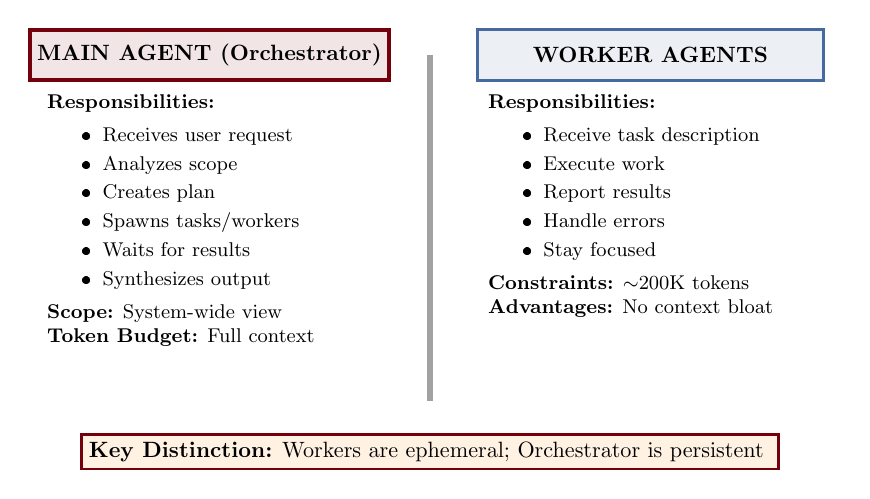
\begin{tikzpicture}[scale=0.8, transform shape]
    % Main Agent Column
    \node[orchestrator, minimum width=5.5cm, minimum height=0.8cm] (main) at (-3.5,3.5) {\textbf{MAIN AGENT (Orchestrator)}};

    \node[anchor=north west, font=\small] at (-6.2,3) {
        \begin{minipage}{5.5cm}
        \textbf{Responsibilities:}
        \begin{itemize}\setlength\itemsep{0pt}
            \item Receives user request
            \item Analyzes scope
            \item Creates plan
            \item Spawns tasks/workers
            \item Waits for results
            \item Synthesizes output
        \end{itemize}
        \textbf{Scope:} System-wide view\\
        \textbf{Token Budget:} Full context
        \end{minipage}
    };

    % Worker Agents Column
    \node[worker, minimum width=5.5cm, minimum height=0.8cm] (work) at (3.5,3.5) {\textbf{WORKER AGENTS}};

    \node[anchor=north west, font=\small] at (0.8,3) {
        \begin{minipage}{5.5cm}
        \textbf{Responsibilities:}
        \begin{itemize}\setlength\itemsep{0pt}
            \item Receive task description
            \item Execute work
            \item Report results
            \item Handle errors
            \item Stay focused
        \end{itemize}
        \textbf{Constraints:} $\sim$200K tokens\\
        \textbf{Advantages:} No context bloat
        \end{minipage}
    };

    % Divider
    \draw[line width=2pt, UofSC50Black] (0,3.5) -- (0,-2);

    % Key distinction
    \node[fill=UofSCSandstorm, draw=UofSCGarnet, line width=1pt, minimum width=10cm, align=center] at (0,-2.8) {
        \textbf{Key Distinction:} Workers are ephemeral; Orchestrator is persistent
    };
\end{tikzpicture}
\end{center}
\end{frame}

% ------------------------------------------------------------
% Slide 4: Why Split Work into Tasks?
% ------------------------------------------------------------
\begin{frame}{Benefits of Task Decomposition}
\begin{columns}[T]
\begin{column}{0.48\textwidth}
\begin{alertblock}{Problem: Single Agent}
\begin{itemize}
    \item Context bloat (token limits)
    \item Loss of focus (too many concerns)
    \item Sequential execution (slow)
    \item Hard to isolate failures
    \item Cannot parallelize
    \item Reduced effectiveness
\end{itemize}
\end{alertblock}
\end{column}
\begin{column}{0.48\textwidth}
\begin{exampleblock}{Solution: Orchestrator + Workers}
\begin{itemize}
    \item Clear token boundaries
    \item Task focus (one thing well)
    \item Parallel execution
    \item Isolated failure handling
    \item Easy to retry failed tasks
    \item Better result quality
    \item Scalability
\end{itemize}
\end{exampleblock}
\end{column}
\end{columns}

\vspace{0.3cm}
\begin{center}

\begin{tikzpicture}
    \node[fill=UofSCGarnet!10, draw=UofSCGarnet, line width=1pt, minimum width=12cm, align=center, font=\bfseries] {
        Key Concept: Task splitting enables parallelization and focus
    };
\end{tikzpicture}
\end{center}
\end{frame}

% ------------------------------------------------------------
% Slide 5: Real-World Analogy
% ------------------------------------------------------------
\begin{frame}{Two-Layer Pattern in Familiar Contexts}
\begin{columns}[T]
\begin{column}{0.48\textwidth}
\begin{center}
\textbf{Construction Project}
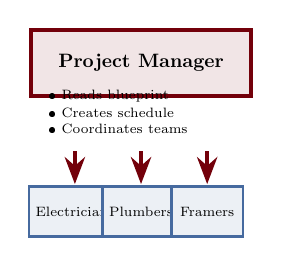
\begin{tikzpicture}[scale=0.7, transform shape]
    \node[orchestrator, minimum width=4cm] (pm) at (0,2) {Project Manager};
    \node[anchor=west, font=\scriptsize] at (-1.8,1.4) {\textbullet\ Reads blueprint};
    \node[anchor=west, font=\scriptsize] at (-1.8,1.1) {\textbullet\ Creates schedule};
    \node[anchor=west, font=\scriptsize] at (-1.8,0.8) {\textbullet\ Coordinates teams};

    \draw[thickarrow] (-1.2,0.4) -- (-1.2,-0.2);
    \draw[thickarrow] (0,0.4) -- (0,-0.2);
    \draw[thickarrow] (1.2,0.4) -- (1.2,-0.2);

    \node[worker, minimum width=1.3cm, font=\scriptsize] at (-1.2,-0.7) {Electricians};
    \node[worker, minimum width=1.3cm, font=\scriptsize] at (0,-0.7) {Plumbers};
    \node[worker, minimum width=1.3cm, font=\scriptsize] at (1.2,-0.7) {Framers};
\end{tikzpicture}
\end{center}
\end{column}
\begin{column}{0.48\textwidth}
\begin{center}
\textbf{Magazine Production}
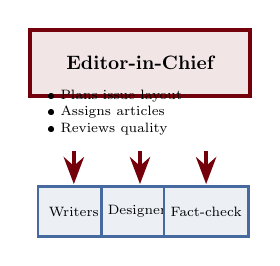
\begin{tikzpicture}[scale=0.7, transform shape]
    \node[orchestrator, minimum width=4cm] (eic) at (0,2) {Editor-in-Chief};
    \node[anchor=west, font=\scriptsize] at (-1.8,1.4) {\textbullet\ Plans issue layout};
    \node[anchor=west, font=\scriptsize] at (-1.8,1.1) {\textbullet\ Assigns articles};
    \node[anchor=west, font=\scriptsize] at (-1.8,0.8) {\textbullet\ Reviews quality};

    \draw[thickarrow] (-1.2,0.4) -- (-1.2,-0.2);
    \draw[thickarrow] (0,0.4) -- (0,-0.2);
    \draw[thickarrow] (1.2,0.4) -- (1.2,-0.2);

    \node[worker, minimum width=1.3cm, font=\scriptsize] at (-1.2,-0.7) {Writers};
    \node[worker, minimum width=1.3cm, font=\scriptsize] at (0,-0.7) {Designers};
    \node[worker, minimum width=1.3cm, font=\scriptsize] at (1.2,-0.7) {Fact-check};
\end{tikzpicture}
\end{center}
\end{column}
\end{columns}

\vspace{0.4cm}
\begin{block}{Universal Pattern}
\begin{itemize}
    \item \textbf{Software:} Tech lead orchestrates backend, frontend, QA teams
    \item \textbf{AI Agents:} Orchestrator agent $\rightarrow$ specialist worker agents
    \item Pattern is timeless and proven at scale
\end{itemize}
\end{block}
\end{frame}

% ------------------------------------------------------------
% Slide 6: When to Use Two-Layer Pattern
% ------------------------------------------------------------
\begin{frame}{When Should You Use Two-Layer Architecture?}
\begin{columns}[T]
\begin{column}{0.55\textwidth}
\begin{center}
\textbf{Decision Tree}
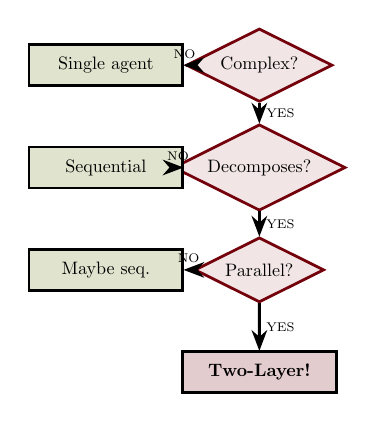
\begin{tikzpicture}[scale=0.65, transform shape]
    \node[decision, minimum width=2.5cm] (q1) at (0,4) {Complex?};
    \node[process, fill=UofSCHorseshoe!20] (a1) at (-3,4) {Single agent};

    \node[decision, minimum width=2.5cm] (q2) at (0,2) {Decomposes?};
    \node[process, fill=UofSCHorseshoe!20] (a2) at (-3,2) {Sequential};

    \node[decision, minimum width=2.5cm] (q3) at (0,0) {Parallel?};
    \node[process, fill=UofSCHorseshoe!20] (a3) at (-3,0) {Maybe seq.};

    \node[process, fill=UofSCGarnet!20, font=\bfseries] (use) at (0,-2) {Two-Layer!};

    \draw[arrow] (q1) -- node[above, font=\scriptsize]{NO} (a1);
    \draw[arrow] (q1) -- node[right, font=\scriptsize]{YES} (q2);
    \draw[arrow] (q2) -- node[above, font=\scriptsize]{NO} (a2);
    \draw[arrow] (q2) -- node[right, font=\scriptsize]{YES} (q3);
    \draw[arrow] (q3) -- node[above, font=\scriptsize]{NO} (a3);
    \draw[arrow] (q3) -- node[right, font=\scriptsize]{YES} (use);
\end{tikzpicture}
\end{center}
\end{column}
\begin{column}{0.45\textwidth}
\begin{block}{Use Two-Layer When:}
\begin{itemize}
    \item Task breaks into 3+ subtasks
    \item Subtasks are independent
    \item Total work $>$ 2--3 hours
    \item Subtasks need specialization
    \item Parallelization saves time
\end{itemize}
\end{block}

\begin{alertblock}{Avoid Two-Layer For:}
\begin{itemize}
    \item Simple, quick tasks ($<$ 1 hour)
    \item Heavy dependencies
    \item Constant decision-making
    \item Minimal context needs
\end{itemize}
\end{alertblock}
\end{column}
\end{columns}
\end{frame}

% ============================================================
% SECTION 2: The Orchestrator-Worker Model
% ============================================================
\section{The Orchestrator-Worker Model}

% ------------------------------------------------------------
% Slide 7: Orchestrator Workflow
% ------------------------------------------------------------
\begin{frame}{The Orchestrator: Strategic Decision-Maker}
\begin{center}
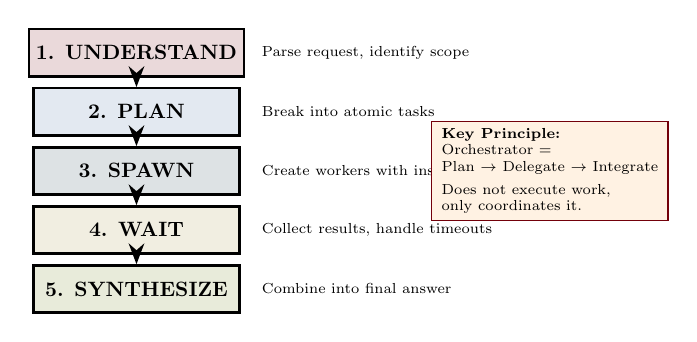
\begin{tikzpicture}[scale=0.75, transform shape]
    % Workflow steps
    \node[process, fill=UofSCGarnet!15, minimum width=3.5cm] (u) at (0,3.5) {\textbf{1. UNDERSTAND}};
    \node[font=\scriptsize, anchor=west] at (2,3.5) {Parse request, identify scope};

    \node[process, fill=UofSCAtlantic!15, minimum width=3.5cm] (p) at (0,2.5) {\textbf{2. PLAN}};
    \node[font=\scriptsize, anchor=west] at (2,2.5) {Break into atomic tasks};

    \node[process, fill=UofSCCongaree!15, minimum width=3.5cm] (s) at (0,1.5) {\textbf{3. SPAWN}};
    \node[font=\scriptsize, anchor=west] at (2,1.5) {Create workers with instructions};

    \node[process, fill=UofSCHoneycomb!15, minimum width=3.5cm] (w) at (0,0.5) {\textbf{4. WAIT}};
    \node[font=\scriptsize, anchor=west] at (2,0.5) {Collect results, handle timeouts};

    \node[process, fill=UofSCHorseshoe!15, minimum width=3.5cm] (sy) at (0,-0.5) {\textbf{5. SYNTHESIZE}};
    \node[font=\scriptsize, anchor=west] at (2,-0.5) {Combine into final answer};

    % Arrows
    \draw[arrow] (u) -- (p);
    \draw[arrow] (p) -- (s);
    \draw[arrow] (s) -- (w);
    \draw[arrow] (w) -- (sy);

    % Side annotations
    \node[draw=UofSCGarnet, fill=UofSCSandstorm, align=left, font=\scriptsize, minimum width=4cm] at (7,1.5) {
        \textbf{Key Principle:}\\
        Orchestrator = \\
        Plan $\rightarrow$ Delegate $\rightarrow$ Integrate\\[3pt]
        Does not execute work,\\
        only coordinates it.
    };
\end{tikzpicture}
\end{center}
\end{frame}

% ------------------------------------------------------------
% Slide 8: Worker Lifecycle
% ------------------------------------------------------------
\begin{frame}{Worker Agents: Focused Executors}
\begin{columns}[T]
\begin{column}{0.5\textwidth}
\begin{center}
\textbf{Worker Lifecycle}
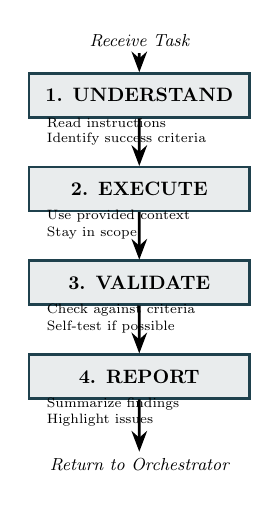
\begin{tikzpicture}[scale=0.7, transform shape]
    \node[font=\small\itshape] (recv) at (0,4.5) {Receive Task};

    \node[task, minimum width=4cm] (t1) at (0,3.5) {\textbf{1. UNDERSTAND}};
    \node[font=\scriptsize, anchor=west] at (-1.8,3) {Read instructions};
    \node[font=\scriptsize, anchor=west] at (-1.8,2.7) {Identify success criteria};

    \node[task, minimum width=4cm] (t2) at (0,1.8) {\textbf{2. EXECUTE}};
    \node[font=\scriptsize, anchor=west] at (-1.8,1.3) {Use provided context};
    \node[font=\scriptsize, anchor=west] at (-1.8,1.0) {Stay in scope};

    \node[task, minimum width=4cm] (t3) at (0,0.1) {\textbf{3. VALIDATE}};
    \node[font=\scriptsize, anchor=west] at (-1.8,-0.4) {Check against criteria};
    \node[font=\scriptsize, anchor=west] at (-1.8,-0.7) {Self-test if possible};

    \node[task, minimum width=4cm] (t4) at (0,-1.6) {\textbf{4. REPORT}};
    \node[font=\scriptsize, anchor=west] at (-1.8,-2.1) {Summarize findings};
    \node[font=\scriptsize, anchor=west] at (-1.8,-2.4) {Highlight issues};

    \node[font=\small\itshape] (ret) at (0,-3.2) {Return to Orchestrator};

    \draw[arrow] (recv) -- (t1);
    \draw[arrow] (t1) -- (t2);
    \draw[arrow] (t2) -- (t3);
    \draw[arrow] (t3) -- (t4);
    \draw[arrow] (t4) -- (ret);
\end{tikzpicture}
\end{center}
\end{column}
\begin{column}{0.5\textwidth}
\begin{block}{Worker Principles}
\begin{itemize}
    \item \textbf{Focused:} One task at a time
    \item \textbf{Disciplined:} Stay within scope
    \item \textbf{Efficient:} Use tokens wisely
    \item \textbf{Clear:} Structured reporting
\end{itemize}
\end{block}

\begin{exampleblock}{Good Worker Behavior}
\begin{itemize}
    \item Reviews exactly assigned files
    \item Does not expand scope
    \item Notes out-of-scope issues
    \item Returns structured results
\end{itemize}
\end{exampleblock}

\vspace{0.2cm}
\textbf{Key:} Worker = Focused execution + Clear reporting
\end{column}
\end{columns}
\end{frame}

% ------------------------------------------------------------
% Slide 9: Communication Flow
% ------------------------------------------------------------
\begin{frame}{How Information Flows Between Layers}
\begin{center}
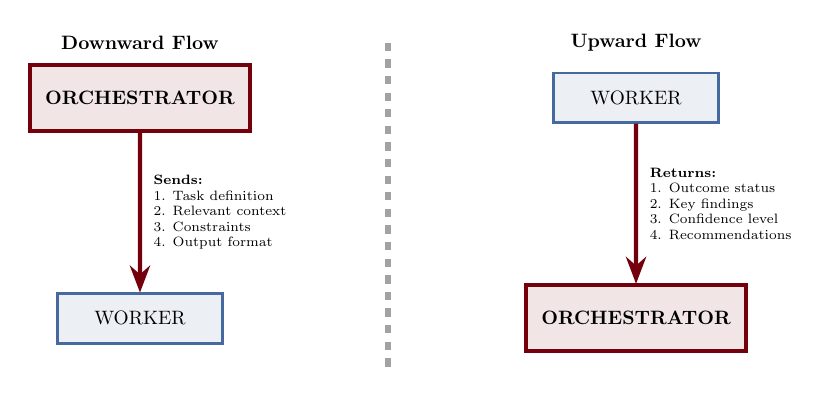
\begin{tikzpicture}[scale=0.7, transform shape]
    % Orchestrator to Worker
    \node[orchestrator, minimum width=4cm] (orch1) at (-4.5,3) {ORCHESTRATOR};
    \node[worker, minimum width=3cm] (work1) at (-4.5,-1) {WORKER};

    \draw[thickarrow] (orch1) -- node[right, font=\scriptsize, align=left, xshift=3pt] {
        \textbf{Sends:}\\
        1. Task definition\\
        2. Relevant context\\
        3. Constraints\\
        4. Output format
    } (work1);

    % Worker to Orchestrator
    \node[worker, minimum width=3cm] (work2) at (4.5,3) {WORKER};
    \node[orchestrator, minimum width=4cm] (orch2) at (4.5,-1) {ORCHESTRATOR};

    \draw[thickarrow] (work2) -- node[right, font=\scriptsize, align=left, xshift=3pt] {
        \textbf{Returns:}\\
        1. Outcome status\\
        2. Key findings\\
        3. Confidence level\\
        4. Recommendations
    } (orch2);

    % Divider
    \draw[line width=2pt, UofSC50Black, dashed] (0,4) -- (0,-2);

    % Labels
    \node[font=\bfseries] at (-4.5,4) {Downward Flow};
    \node[font=\bfseries] at (4.5,4) {Upward Flow};
\end{tikzpicture}
\end{center}

\vspace{0.2cm}
\begin{block}{Communication Principle}
Like API contracts: clear input specification and output schema for easy synthesis
\end{block}
\end{frame}

% ------------------------------------------------------------
% Slide 10: Result Synthesis
% ------------------------------------------------------------
\begin{frame}{Combining Worker Results Into Final Output}
\begin{center}
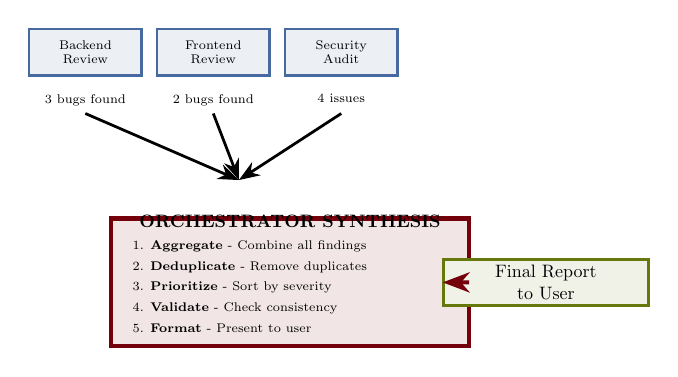
\begin{tikzpicture}[scale=0.65, transform shape]
    % Workers reporting
    \node[worker, minimum width=2.2cm, font=\scriptsize] (w1) at (-4,3) {Backend\\Review};
    \node[worker, minimum width=2.2cm, font=\scriptsize] (w2) at (-1.5,3) {Frontend\\Review};
    \node[worker, minimum width=2.2cm, font=\scriptsize] (w3) at (1,3) {Security\\Audit};

    % Results
    \node[font=\scriptsize, anchor=north] at (-4,2.3) {3 bugs found};
    \node[font=\scriptsize, anchor=north] at (-1.5,2.3) {2 bugs found};
    \node[font=\scriptsize, anchor=north] at (1,2.3) {4 issues};

    % Arrows to synthesis
    \draw[arrow] (-4,1.8) -- (-1,0.5);
    \draw[arrow] (-1.5,1.8) -- (-1,0.5);
    \draw[arrow] (1,1.8) -- (-1,0.5);

    % Synthesis box
    \node[orchestrator, minimum width=7cm, minimum height=2.5cm] (synth) at (0,-1.5) {};
    \node[font=\bfseries] at (0,-0.3) {ORCHESTRATOR SYNTHESIS};

    \node[font=\scriptsize, anchor=west] at (-3.2,-0.8) {1. \textbf{Aggregate} - Combine all findings};
    \node[font=\scriptsize, anchor=west] at (-3.2,-1.2) {2. \textbf{Deduplicate} - Remove duplicates};
    \node[font=\scriptsize, anchor=west] at (-3.2,-1.6) {3. \textbf{Prioritize} - Sort by severity};
    \node[font=\scriptsize, anchor=west] at (-3.2,-2.0) {4. \textbf{Validate} - Check consistency};
    \node[font=\scriptsize, anchor=west] at (-3.2,-2.4) {5. \textbf{Format} - Present to user};

    % Final output
    \node[result, minimum width=4cm] (out) at (5,-1.5) {Final Report\\to User};
    \draw[thickarrow] (3.5,-1.5) -- (out);
\end{tikzpicture}
\end{center}

\textbf{Key:} Synthesis = Integration + Analysis + Decision-Making
\end{frame}

% ------------------------------------------------------------
% Slide 11: Dependency Patterns
% ------------------------------------------------------------
\begin{frame}{Handling Task Dependencies}
\begin{columns}[T]
\begin{column}{0.33\textwidth}
\begin{center}
\textbf{Pattern 1: Parallel}\\[5pt]
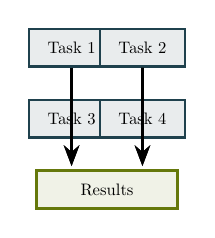
\begin{tikzpicture}[scale=0.6, transform shape]
    \node[task] (t1) at (0,2) {Task 1};
    \node[task] (t2) at (1.5,2) {Task 2};
    \node[task] (t3) at (0,0.5) {Task 3};
    \node[task] (t4) at (1.5,0.5) {Task 4};

    \node[result, minimum width=3cm] (r) at (0.75,-1) {Results};

    \draw[arrow] (t1) -- (0,-0.5);
    \draw[arrow] (t2) -- (1.5,-0.5);
    \draw[arrow] (t3) -- (0,-0.5);
    \draw[arrow] (t4) -- (1.5,-0.5);
\end{tikzpicture}
\\[5pt]
\scriptsize No dependencies\\All run simultaneously
\end{center}
\end{column}
\begin{column}{0.33\textwidth}
\begin{center}
\textbf{Pattern 2: Linear}\\[5pt]
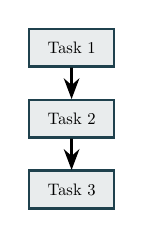
\begin{tikzpicture}[scale=0.6, transform shape]
    \node[task] (t1) at (0.75,2.5) {Task 1};
    \node[task] (t2) at (0.75,1) {Task 2};
    \node[task] (t3) at (0.75,-0.5) {Task 3};

    \draw[arrow] (t1) -- (t2);
    \draw[arrow] (t2) -- (t3);
\end{tikzpicture}
\\[5pt]
\scriptsize Sequential deps\\Must run in order
\end{center}
\end{column}
\begin{column}{0.33\textwidth}
\begin{center}
\textbf{Pattern 3: Tree}\\[5pt]
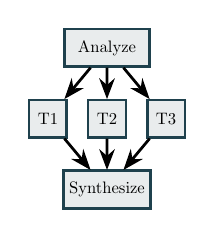
\begin{tikzpicture}[scale=0.6, transform shape]
    \node[task] (a) at (0.75,2.5) {Analyze};
    \node[task, minimum width=0.8cm] (t1) at (-0.5,1) {T1};
    \node[task, minimum width=0.8cm] (t2) at (0.75,1) {T2};
    \node[task, minimum width=0.8cm] (t3) at (2,1) {T3};
    \node[task] (s) at (0.75,-0.5) {Synthesize};

    \draw[arrow] (a) -- (t1);
    \draw[arrow] (a) -- (t2);
    \draw[arrow] (a) -- (t3);
    \draw[arrow] (t1) -- (s);
    \draw[arrow] (t2) -- (s);
    \draw[arrow] (t3) -- (s);
\end{tikzpicture}
\\[5pt]
\scriptsize Mixed parallel\\and sequential
\end{center}
\end{column}
\end{columns}

\vspace{0.3cm}
\begin{block}{Dependency Resolution}
\begin{itemize}
    \item Identify dependencies early in planning phase
    \item Run independent tasks in parallel; only serialize when necessary
    \item Use completed results to inform later tasks
\end{itemize}
\end{block}
\end{frame}

% ------------------------------------------------------------
% Slide 12: Error Handling
% ------------------------------------------------------------
\begin{frame}{Managing Failures in the Two-Layer System}
\begin{columns}[T]
\begin{column}{0.5\textwidth}
\begin{center}
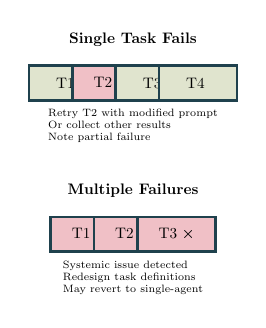
\begin{tikzpicture}[scale=0.55, transform shape]
    % Scenario 1
    \node[font=\bfseries] at (0,4.5) {Single Task Fails};
    \node[task, fill=UofSCHorseshoe!20] (t1) at (-1.5,3.5) {T1 \checkmark};
    \node[task, fill=UofSCRose!30] (t2) at (-0.5,3.5) {T2 \texttimes};
    \node[task, fill=UofSCHorseshoe!20] (t3) at (0.5,3.5) {T3 \checkmark};
    \node[task, fill=UofSCHorseshoe!20] (t4) at (1.5,3.5) {T4 \checkmark};

    \node[font=\scriptsize, align=left] at (0,2.5) {
        Retry T2 with modified prompt\\
        Or collect other results\\
        Note partial failure
    };

    % Scenario 2
    \node[font=\bfseries] at (0,1) {Multiple Failures};
    \node[task, fill=UofSCRose!30] (t1b) at (-1,0) {T1 \texttimes};
    \node[task, fill=UofSCRose!30] (t2b) at (0,0) {T2 \texttimes};
    \node[task, fill=UofSCRose!30] (t3b) at (1,0) {T3 \texttimes};

    \node[font=\scriptsize, align=left] at (0,-1) {
        Systemic issue detected\\
        Redesign task definitions\\
        May revert to single-agent
    };
\end{tikzpicture}
\end{center}
\end{column}
\begin{column}{0.5\textwidth}
\begin{block}{Error Scenarios}
\begin{description}
    \item[Single Failure] Retry or use partial results
    \item[Timeout] Worker too slow; terminate and retry
    \item[Systemic] All fail; indicates design problem
\end{description}
\end{block}

\begin{exampleblock}{Recovery Strategies}
\begin{itemize}
    \item Retry with simpler prompt
    \item Add more context/guidance
    \item Break into smaller pieces
    \item Fallback to single-agent
\end{itemize}
\end{exampleblock}

\textbf{Key:} Failures are isolated; orchestrator adapts
\end{column}
\end{columns}
\end{frame}

% ============================================================
% SECTION 3: Task vs Subagent Distinction
% ============================================================
\section{Tasks vs Subagents}

% ------------------------------------------------------------
% Slide 13: Comparison Matrix
% ------------------------------------------------------------
\begin{frame}{Two Ways to Delegate Work}
\begin{center}
\begin{tabular}{>{\bfseries}l p{4.5cm} p{4.5cm}}
\toprule
\textbf{Aspect} & \textbf{TASKS} & \textbf{SUBAGENTS} \\
\midrule
Lifetime & Ephemeral, one-off job & Persistent throughout sequence \\
\addlinespace
Token Budget & $\sim$200K per task, no carryover & Fresh budget per interaction \\
\addlinespace
State & Stateless, no memory & Maintains state, remembers \\
\addlinespace
Init Cost & Quick, minimal overhead & Slower, more setup \\
\addlinespace
Ideal For & Isolated, parallelizable work & Iterative, multi-turn work \\
\addlinespace
Concurrency & Up to 10 simultaneous & Typically 1--3 sequential \\
\bottomrule
\end{tabular}
\end{center}

\vspace{0.3cm}
\begin{block}{Key Distinction}
\textbf{Tasks} = Stateless one-offs for parallel execution\\
\textbf{Subagents} = Persistent specialists with memory for iterative work
\end{block}
\end{frame}

% ------------------------------------------------------------
% Slide 14: Task Characteristics
% ------------------------------------------------------------
\begin{frame}{Tasks: Lightweight, Stateless Execution}
\begin{columns}[T]
\begin{column}{0.5\textwidth}
\begin{center}
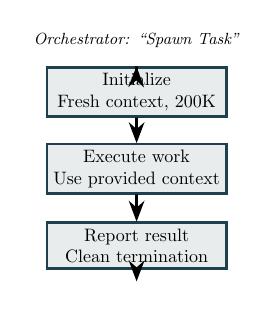
\begin{tikzpicture}[scale=0.65, transform shape]
    \node[font=\small\itshape] at (0,4) {Orchestrator: ``Spawn Task''};

    \node[task, minimum width=3.5cm] (init) at (0,3) {Initialize\\Fresh context, 200K};

    \node[task, minimum width=3.5cm] (exec) at (0,1.5) {Execute work\\Use provided context};

    \node[task, minimum width=3.5cm] (rep) at (0,0) {Report result\\Clean termination};

    \draw[arrow] (0,3.5) -- (init);
    \draw[arrow] (init) -- (exec);
    \draw[arrow] (exec) -- (rep);
    \draw[arrow] (rep) -- (0,-0.7);
\end{tikzpicture}
\end{center}
\end{column}
\begin{column}{0.5\textwidth}
\begin{block}{Ideal Task Characteristics}
\begin{itemize}
    \item Self-contained work
    \item Clear input $\rightarrow$ output
    \item No previous task dependency
    \item Can be parallelized
    \item Execution $<$ 5 minutes
    \item Result is final (no back-and-forth)
\end{itemize}
\end{block}

\begin{exampleblock}{Best For}
Analyzing files, running tests, generating docs, code reviews, data processing
\end{exampleblock}
\end{column}
\end{columns}

\vspace{0.2cm}
\textbf{Advantage:} Fresh context means no bloat; optimized for parallelization
\end{frame}

% ------------------------------------------------------------
% Slide 15: Subagent Characteristics
% ------------------------------------------------------------
\begin{frame}{Subagents: Persistent, Stateful Partners}
\begin{columns}[T]
\begin{column}{0.5\textwidth}
\begin{center}
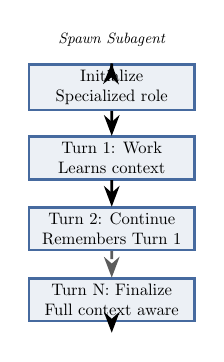
\begin{tikzpicture}[scale=0.6, transform shape]
    \node[font=\small\itshape] at (0,4.5) {Spawn Subagent};

    \node[worker, minimum width=3.5cm] (init) at (0,3.5) {Initialize\\Specialized role};

    \node[worker, minimum width=3.5cm] (t1) at (0,2) {Turn 1: Work\\Learns context};

    \node[worker, minimum width=3.5cm] (t2) at (0,0.5) {Turn 2: Continue\\Remembers Turn 1};

    \node[worker, minimum width=3.5cm] (tn) at (0,-1) {Turn N: Finalize\\Full context aware};

    \draw[arrow] (0,4) -- (init);
    \draw[arrow] (init) -- (t1);
    \draw[arrow] (t1) -- (t2);
    \draw[dashedarrow] (t2) -- (tn);
    \draw[arrow] (tn) -- (0,-1.7);
\end{tikzpicture}
\end{center}
\end{column}
\begin{column}{0.5\textwidth}
\begin{block}{Ideal Subagent Work}
\begin{itemize}
    \item Iterative problem solving
    \item Multi-turn interactions
    \item Specialist roles
    \item Benefits from context growth
    \item Related decisions over time
\end{itemize}
\end{block}

\begin{exampleblock}{Best For}
Architecture design, writing with feedback, complex debugging, feature implementation cycles
\end{exampleblock}
\end{column}
\end{columns}

\vspace{0.2cm}
\textbf{Advantage:} Remembers prior interactions, builds sophisticated understanding
\end{frame}

% ------------------------------------------------------------
% Slide 16: Decision Tree
% ------------------------------------------------------------
\begin{frame}{Decision Tree: Tasks or Subagents?}
\begin{columns}[T]
\begin{column}{0.55\textwidth}
\begin{center}
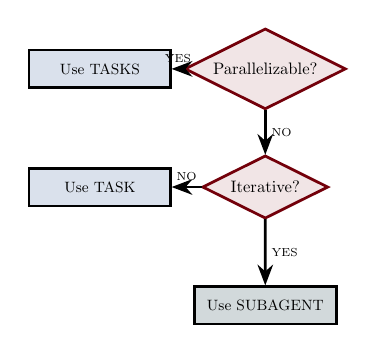
\begin{tikzpicture}[scale=0.6, transform shape]
    \node[decision] (q1) at (0,3) {Parallelizable?};

    \node[process, fill=UofSCAtlantic!20, font=\small] (task1) at (-3.5,3) {Use TASKS};

    \node[decision] (q2) at (0,0.5) {Iterative?};

    \node[process, fill=UofSCAtlantic!20, font=\small] (task2) at (-3.5,0.5) {Use TASK};

    \node[process, fill=UofSCCongaree!20, font=\small] (sub) at (0,-2) {Use SUBAGENT};

    \draw[arrow] (q1) -- node[above, font=\scriptsize]{YES} (task1);
    \draw[arrow] (q1) -- node[right, font=\scriptsize]{NO} (q2);
    \draw[arrow] (q2) -- node[above, font=\scriptsize]{NO} (task2);
    \draw[arrow] (q2) -- node[right, font=\scriptsize]{YES} (sub);
\end{tikzpicture}
\end{center}
\end{column}
\begin{column}{0.45\textwidth}
\begin{block}{Quick Reference}
\begin{tabular}{ll}
\textbf{Task} & \textbf{Subagent} \\
\midrule
Code review & Code architect \\
Test file X & Integrate \& test \\
Security scan & Design protocol \\
Analyze data & Data strategy \\
Generate docs & Doc specialist \\
\end{tabular}
\end{block}

\vspace{0.3cm}
\textbf{Rule of Thumb:}\\
Parallelizable = Tasks\\
Iterative = Subagents
\end{column}
\end{columns}
\end{frame}

% ============================================================
% SECTION 4: Claude Code Task Tool
% ============================================================
\section{Claude Code Task Tool}

% ------------------------------------------------------------
% Slide 17: Task Tool Overview
% ------------------------------------------------------------
\begin{frame}{The Task Tool: Spawning Worker Agents}
\begin{columns}[T]
\begin{column}{0.55\textwidth}
\begin{block}{What It Is}
\begin{itemize}
    \item Built-in command for parallel agents
    \item Terminal-based, integrated
    \item Handles context isolation
    \item Manages constraints and execution
\end{itemize}
\end{block}

\begin{exampleblock}{Key Features}
\begin{itemize}
    \item Parallel execution (up to 10 concurrent)
    \item Automatic context isolation
    \item Result collection and buffering
    \item Timeout management
    \item Structured output format
\end{itemize}
\end{exampleblock}
\end{column}
\begin{column}{0.45\textwidth}
\begin{block}{Basic Syntax}
\texttt{\textcolor{UofSCGarnet}{task:} "instruction" [options]}
\end{block}

\begin{exampleblock}{Example}
{\scriptsize\ttfamily
\textcolor{UofSCGarnet}{task:} "Review auth module"\\
\hspace{1em}--context="src/auth.py"\\
\hspace{1em}--timeout=300\\
\hspace{1em}--name="auth-review"
}
\end{exampleblock}

\vspace{0.3cm}
\textbf{Key Concept:}\\
Task tool = Built-in parallelization mechanism
\end{column}
\end{columns}
\end{frame}

% ------------------------------------------------------------
% Slide 18: Task Parameters
% ------------------------------------------------------------
\begin{frame}[fragile]{Task Tool Parameters and Options}
\begin{columns}[T]
\begin{column}{0.5\textwidth}
\begin{block}{Complete Syntax}
\begin{semiverbatim}\scriptsize
\textcolor{UofSCGarnet}{task:} "Primary instruction"
  --name="task-identifier"
  --context="file or glob"
  --timeout=300
  --output-format="json"
  --priority="normal"
\end{semiverbatim}
\end{block}

\begin{block}{Parameter Details}
\begin{description}
    \item[Instruction] What to do (required)
    \item[Name] Identifier for tracking
    \item[Context] Files to provide
    \item[Timeout] Max seconds (120--600)
    \item[Output] json, text, markdown
\end{description}
\end{block}
\end{column}
\begin{column}{0.5\textwidth}
\begin{exampleblock}{Full Example}
\begin{semiverbatim}\scriptsize
\textcolor{UofSCGarnet}{task:} "Find security vulns"
  --name="security-audit"
  --context="src/auth/*.py"
  --timeout=300
  --output-format="json"
  --priority="high"
\end{semiverbatim}
\end{exampleblock}

\begin{alertblock}{Best Practice}
Provide only relevant context. If task reviews \texttt{auth.py}, provide just that file.
\end{alertblock}
\end{column}
\end{columns}
\end{frame}

% ------------------------------------------------------------
% Slide 19: Parallel Spawning
% ------------------------------------------------------------
\begin{frame}{Running Tasks in Parallel}
\begin{columns}[T]
\begin{column}{0.5\textwidth}
\begin{center}
\textbf{Sequential (Slow)}
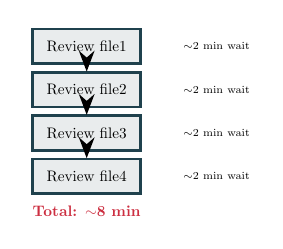
\begin{tikzpicture}[scale=0.55, transform shape]
    \node[task, minimum width=2.5cm] (t1) at (0,3) {Review file1};
    \node[font=\scriptsize] at (3,3) {$\sim$2 min wait};
    \node[task, minimum width=2.5cm] (t2) at (0,2) {Review file2};
    \node[font=\scriptsize] at (3,2) {$\sim$2 min wait};
    \node[task, minimum width=2.5cm] (t3) at (0,1) {Review file3};
    \node[font=\scriptsize] at (3,1) {$\sim$2 min wait};
    \node[task, minimum width=2.5cm] (t4) at (0,0) {Review file4};
    \node[font=\scriptsize] at (3,0) {$\sim$2 min wait};

    \draw[arrow] (t1) -- (t2);
    \draw[arrow] (t2) -- (t3);
    \draw[arrow] (t3) -- (t4);

    \node[font=\bfseries, text=UofSCRose] at (0,-0.8) {Total: $\sim$8 min};
\end{tikzpicture}
\end{center}
\end{column}
\begin{column}{0.5\textwidth}
\begin{center}
\textbf{Parallel (Fast)}
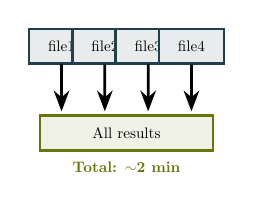
\begin{tikzpicture}[scale=0.55, transform shape]
    \node[task, minimum width=1.5cm] (t1) at (-1.5,2) {file1};
    \node[task, minimum width=1.5cm] (t2) at (-0.5,2) {file2};
    \node[task, minimum width=1.5cm] (t3) at (0.5,2) {file3};
    \node[task, minimum width=1.5cm] (t4) at (1.5,2) {file4};

    \draw[arrow] (t1) -- (-1.5,0.5);
    \draw[arrow] (t2) -- (-0.5,0.5);
    \draw[arrow] (t3) -- (0.5,0.5);
    \draw[arrow] (t4) -- (1.5,0.5);

    \node[result, minimum width=4cm] (r) at (0,0) {All results};

    \node[font=\bfseries, text=UofSCHorseshoe] at (0,-0.8) {Total: $\sim$2 min};
\end{tikzpicture}
\end{center}
\end{column}
\end{columns}

\vspace{0.3cm}
\begin{block}{Parallelization Efficiency}
\begin{itemize}
    \item \textbf{Constraint:} Maximum 10 concurrent tasks
    \item \textbf{Speedup:} N similar tasks take $\sim$1/N time
    \item \textbf{Strategy:} Spawn all at once, wait for batch completion
\end{itemize}
\end{block}
\end{frame}

% ------------------------------------------------------------
% Slide 20: Context Isolation
% ------------------------------------------------------------
\begin{frame}{Token Budget and Context Isolation}
\begin{center}
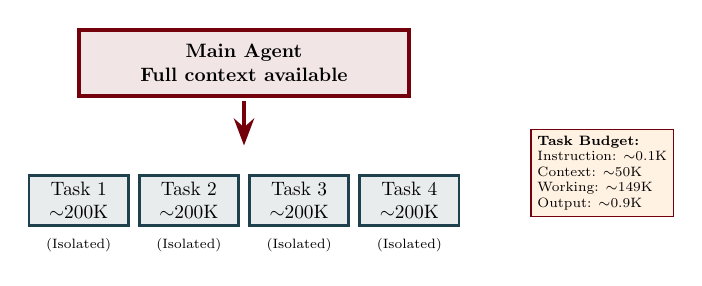
\begin{tikzpicture}[scale=0.7, transform shape]
    % Main agent
    \node[orchestrator, minimum width=6cm] (main) at (0,3) {Main Agent\\Full context available};

    % Arrow down
    \draw[thickarrow] (0,2.3) -- (0,1.5);

    % Tasks
    \node[task] (t1) at (-3,0.5) {Task 1\\$\sim$200K};
    \node[task] (t2) at (-1,0.5) {Task 2\\$\sim$200K};
    \node[task] (t3) at (1,0.5) {Task 3\\$\sim$200K};
    \node[task] (t4) at (3,0.5) {Task 4\\$\sim$200K};

    % Labels
    \node[font=\scriptsize] at (-3,-0.3) {(Isolated)};
    \node[font=\scriptsize] at (-1,-0.3) {(Isolated)};
    \node[font=\scriptsize] at (1,-0.3) {(Isolated)};
    \node[font=\scriptsize] at (3,-0.3) {(Isolated)};

    % Budget breakdown
    \node[draw=UofSCGarnet, fill=UofSCSandstorm, align=left, font=\scriptsize] at (6.5,1) {
        \textbf{Task Budget:}\\
        Instruction: $\sim$0.1K\\
        Context: $\sim$50K\\
        Working: $\sim$149K\\
        Output: $\sim$0.9K
    };
\end{tikzpicture}
\end{center}

\vspace{0.2cm}
\begin{columns}[T]
\begin{column}{0.48\textwidth}
\begin{exampleblock}{Good Context}
\texttt{--context="src/auth.py"} [5K]\\
Leaves plenty for thinking
\end{exampleblock}
\end{column}
\begin{column}{0.48\textwidth}
\begin{alertblock}{Bad Context}
\texttt{--context="src/**/*.py"} [500K]\\
Exceeds budget, will fail
\end{alertblock}
\end{column}
\end{columns}
\end{frame}

% ------------------------------------------------------------
% Slide 21: Concurrency Limits
% ------------------------------------------------------------
\begin{frame}{Concurrency Limits and Batching}
\begin{columns}[T]
\begin{column}{0.5\textwidth}
\begin{center}
\textbf{Maximum 10 Concurrent}
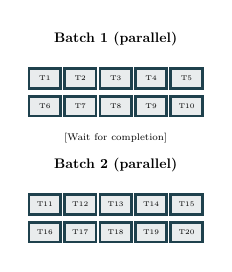
\begin{tikzpicture}[scale=0.5, transform shape]
    % Batch 1
    \node[font=\bfseries] at (0,4) {Batch 1 (parallel)};
    \foreach \i in {1,...,5} {
        \node[task, minimum width=0.8cm, minimum height=0.5cm, font=\tiny] at ({(\i-3)*0.9},3) {T\i};
    }
    \foreach \i in {6,...,10} {
        \node[task, minimum width=0.8cm, minimum height=0.5cm, font=\tiny] at ({(\i-8)*0.9},2.3) {T\i};
    }

    \node[font=\scriptsize] at (0,1.5) {[Wait for completion]};

    % Batch 2
    \node[font=\bfseries] at (0,0.8) {Batch 2 (parallel)};
    \foreach \i in {11,...,15} {
        \node[task, minimum width=0.8cm, minimum height=0.5cm, font=\tiny] at ({(\i-13)*0.9},-0.2) {T\i};
    }
    \foreach \i in {16,...,20} {
        \node[task, minimum width=0.8cm, minimum height=0.5cm, font=\tiny] at ({(\i-18)*0.9},-0.9) {T\i};
    }
\end{tikzpicture}
\end{center}
\end{column}
\begin{column}{0.5\textwidth}
\begin{block}{Batching Strategy}
50 functions to review:
\begin{itemize}
    \item Batch 1: Func 1--10 (2 min)
    \item Batch 2: Func 11--20 (2 min)
    \item Batch 3: Func 21--30 (2 min)
    \item Batch 4: Func 31--40 (2 min)
    \item Batch 5: Func 41--50 (2 min)
\end{itemize}
\textbf{Total:} 10 min vs 100 min sequential
\end{block}
\end{column}
\end{columns}

\vspace{0.2cm}
\begin{alertblock}{Constraint}
Hard limit of 10 concurrent tasks. If $>$10 needed, batch sequentially.
\end{alertblock}
\end{frame}

% ------------------------------------------------------------
% Slide 22: Result Collection
% ------------------------------------------------------------
\begin{frame}{Handling Task Results}
\begin{columns}[T]
\begin{column}{0.5\textwidth}
\begin{block}{Result Structure}
{\scriptsize\ttfamily
\{\\
\hspace{1em}"task\_id": "t1",\\
\hspace{1em}"status": "success",\\
\hspace{1em}"output": "result",\\
\hspace{1em}"exec\_time": 45,\\
\hspace{1em}"tokens\_used": 12500\\
\}
}
\end{block}

\begin{block}{Status Values}
\begin{description}
    \item[success] Process normally
    \item[timeout] Ran too long
    \item[error] Something failed
\end{description}
\end{block}
\end{column}
\begin{column}{0.5\textwidth}
\begin{center}
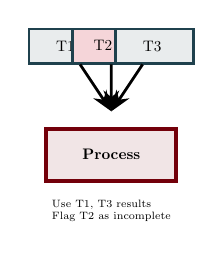
\begin{tikzpicture}[scale=0.55, transform shape]
    \node[task] (t1) at (-1,3) {T1 \checkmark};
    \node[task, fill=UofSCRose!20] (t2) at (0,3) {T2 \texttimes};
    \node[task] (t3) at (1,3) {T3 \checkmark};

    \draw[arrow] (t1) -- (0,1.5);
    \draw[arrow] (t2) -- (0,1.5);
    \draw[arrow] (t3) -- (0,1.5);

    \node[orchestrator, minimum width=3cm] (orch) at (0,0.5) {Process};

    \node[font=\scriptsize, align=left] at (0,-0.8) {
        Use T1, T3 results\\
        Flag T2 as incomplete
    };
\end{tikzpicture}
\end{center}

\textbf{Key:} Collect all results, handle failures gracefully
\end{column}
\end{columns}
\end{frame}

% ============================================================
% SECTION 5: Two-Layer in Other Tools
% ============================================================
\section{Pattern Across Tools}

% ------------------------------------------------------------
% Slide 23: Aider
% ------------------------------------------------------------
\begin{frame}{Two-Layer Pattern in Aider}
\begin{columns}[T]
\begin{column}{0.55\textwidth}
\begin{center}
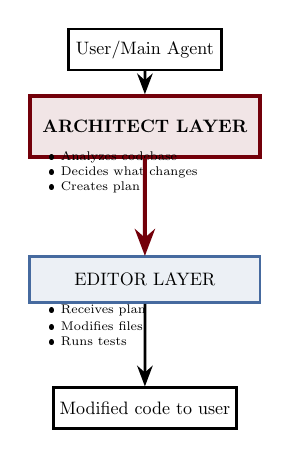
\begin{tikzpicture}[scale=0.65, transform shape]
    \node[process] (user) at (0,4) {User/Main Agent};

    \node[orchestrator, minimum width=4.5cm] (arch) at (0,2.5) {ARCHITECT LAYER};
    \node[font=\scriptsize, anchor=west] at (-2,1.9) {\textbullet\ Analyzes codebase};
    \node[font=\scriptsize, anchor=west] at (-2,1.6) {\textbullet\ Decides what changes};
    \node[font=\scriptsize, anchor=west] at (-2,1.3) {\textbullet\ Creates plan};

    \node[worker, minimum width=4.5cm] (edit) at (0,-0.5) {EDITOR LAYER};
    \node[font=\scriptsize, anchor=west] at (-2,-1.1) {\textbullet\ Receives plan};
    \node[font=\scriptsize, anchor=west] at (-2,-1.4) {\textbullet\ Modifies files};
    \node[font=\scriptsize, anchor=west] at (-2,-1.7) {\textbullet\ Runs tests};

    \node[process] (out) at (0,-3) {Modified code to user};

    \draw[arrow] (user) -- (arch);
    \draw[thickarrow] (arch) -- (edit);
    \draw[arrow] (edit) -- (out);
\end{tikzpicture}
\end{center}
\end{column}
\begin{column}{0.45\textwidth}
\begin{block}{Aider Roles}
\begin{description}
    \item[Architect] Analyzes, plans, decides approach
    \item[Editor] Implements specified changes
\end{description}
\end{block}

\begin{exampleblock}{Analogy to Claude Code}
\begin{itemize}
    \item Architect = Orchestrator
    \item Editor = Task Worker
    \item Both use Claude LLM
\end{itemize}
\end{exampleblock}

\textbf{Key:} Separation of thinking vs doing
\end{column}
\end{columns}
\end{frame}

% ------------------------------------------------------------
% Slide 24: OpenHands
% ------------------------------------------------------------
\begin{frame}{Delegation Pattern in OpenHands}
\begin{center}
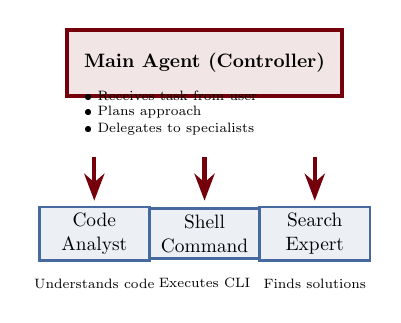
\begin{tikzpicture}[scale=0.7, transform shape]
    \node[orchestrator, minimum width=5cm] (main) at (0,2.5) {Main Agent (Controller)};
    \node[font=\scriptsize, anchor=west] at (-2.3,1.9) {\textbullet\ Receives task from user};
    \node[font=\scriptsize, anchor=west] at (-2.3,1.6) {\textbullet\ Plans approach};
    \node[font=\scriptsize, anchor=west] at (-2.3,1.3) {\textbullet\ Delegates to specialists};

    \draw[thickarrow] (-2,0.8) -- (-2,0);
    \draw[thickarrow] (0,0.8) -- (0,0);
    \draw[thickarrow] (2,0.8) -- (2,0);

    \node[worker] (code) at (-2,-0.6) {Code\\Analyst};
    \node[worker] (shell) at (0,-0.6) {Shell\\Command};
    \node[worker] (search) at (2,-0.6) {Search\\Expert};

    \node[font=\scriptsize] at (-2,-1.5) {Understands code};
    \node[font=\scriptsize] at (0,-1.5) {Executes CLI};
    \node[font=\scriptsize] at (2,-1.5) {Finds solutions};
\end{tikzpicture}
\end{center}

\begin{block}{Specialist Pattern}
\begin{itemize}
    \item Each agent handles specific domain
    \item Controller routes tasks to appropriate specialists
    \item New specialists can be added without changing core
\end{itemize}
\end{block}
\end{frame}

% ------------------------------------------------------------
% Slide 25: Universal Pattern
% ------------------------------------------------------------
\begin{frame}{Common Two-Layer Patterns Across AI Tools}
\begin{center}
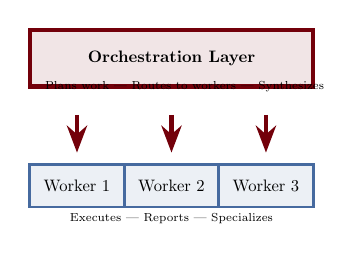
\begin{tikzpicture}[scale=0.6, transform shape]
    % Generic pattern
    \node[orchestrator, minimum width=6cm] (orch) at (0,3) {Orchestration Layer};
    \node[font=\scriptsize, anchor=west] at (-2.8,2.4) {Plans work | Routes to workers | Synthesizes};

    \draw[thickarrow] (-2,1.8) -- (-2,1);
    \draw[thickarrow] (0,1.8) -- (0,1);
    \draw[thickarrow] (2,1.8) -- (2,1);

    \node[worker] (w1) at (-2,0.3) {Worker 1};
    \node[worker] (w2) at (0,0.3) {Worker 2};
    \node[worker] (w3) at (2,0.3) {Worker 3};
    \node[font=\scriptsize] at (0,-0.4) {Executes | Reports | Specializes};
\end{tikzpicture}
\end{center}

\begin{columns}[T]
\begin{column}{0.48\textwidth}
\begin{block}{Why This Pattern Works}
\begin{itemize}
    \item Separation of concerns
    \item Specialists $>$ generalists
    \item Easy to scale (add workers)
    \item Failure isolation
    \item Parallelization
\end{itemize}
\end{block}
\end{column}
\begin{column}{0.48\textwidth}
\begin{exampleblock}{Tool Comparison}
\begin{tabular}{ll}
\textbf{Tool} & \textbf{Pattern} \\
\midrule
Claude Code & Main $\rightarrow$ Tasks \\
Aider & Architect $\rightarrow$ Editor \\
OpenHands & Controller $\rightarrow$ Agents \\
Copilot & Pipeline stages \\
\end{tabular}
\end{exampleblock}
\end{column}
\end{columns}
\end{frame}

% ============================================================
% SECTION 6: Practical Examples
% ============================================================
\section{Practical Examples}

% ------------------------------------------------------------
% Slide 26: Code Review Example
% ------------------------------------------------------------
\begin{frame}{Example: Multi-Specialist Code Review}
\begin{center}
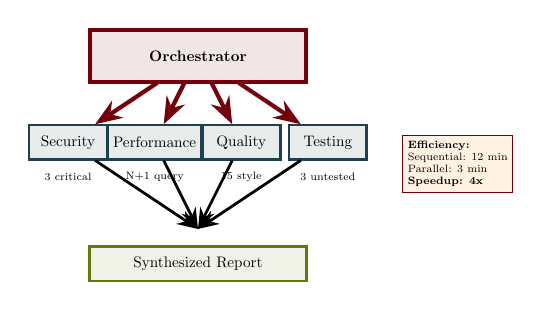
\begin{tikzpicture}[scale=0.55, transform shape]
    \node[orchestrator, minimum width=5cm] (orch) at (0,4) {Orchestrator};

    % Task spawning
    \node[task] (t1) at (-3,2) {Security};
    \node[task] (t2) at (-1,2) {Performance};
    \node[task] (t3) at (1,2) {Quality};
    \node[task] (t4) at (3,2) {Testing};

    \draw[thickarrow] (orch) -- (t1);
    \draw[thickarrow] (orch) -- (t2);
    \draw[thickarrow] (orch) -- (t3);
    \draw[thickarrow] (orch) -- (t4);

    % Results
    \node[font=\scriptsize] at (-3,1.2) {3 critical};
    \node[font=\scriptsize] at (-1,1.2) {N+1 query};
    \node[font=\scriptsize] at (1,1.2) {15 style};
    \node[font=\scriptsize] at (3,1.2) {3 untested};

    % Synthesis
    \draw[arrow] (t1) -- (0,0);
    \draw[arrow] (t2) -- (0,0);
    \draw[arrow] (t3) -- (0,0);
    \draw[arrow] (t4) -- (0,0);

    \node[result, minimum width=5cm] (synth) at (0,-0.8) {Synthesized Report};

    % Efficiency
    \node[draw=UofSCGarnet, fill=UofSCSandstorm, font=\scriptsize, align=left] at (6,1.5) {
        \textbf{Efficiency:}\\
        Sequential: 12 min\\
        Parallel: 3 min\\
        \textbf{Speedup: 4x}
    };
\end{tikzpicture}
\end{center}

\begin{block}{Pattern Benefits}
\begin{itemize}
    \item Each specialist focuses on one domain
    \item 4 experts work simultaneously on same code
    \item Combined findings into prioritized report
\end{itemize}
\end{block}
\end{frame}

% ------------------------------------------------------------
% Slide 27: Feature Implementation
% ------------------------------------------------------------
\begin{frame}{Example: Building a Complex Feature}
\begin{center}
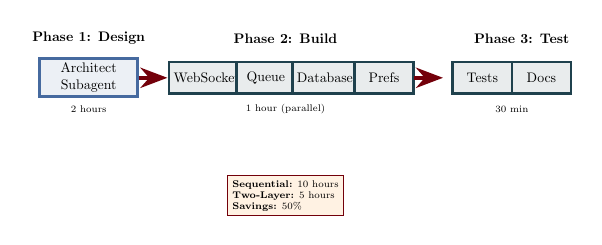
\begin{tikzpicture}[scale=0.5, transform shape]
    % Phase 1
    \node[font=\bfseries] at (-5,3.5) {Phase 1: Design};
    \node[worker, minimum width=2.5cm] (arch) at (-5,2.5) {Architect\\Subagent};
    \node[font=\scriptsize] at (-5,1.7) {2 hours};

    % Phase 2
    \node[font=\bfseries] at (0,3.5) {Phase 2: Build};
    \node[task, minimum width=1.5cm] (c1) at (-2,2.5) {WebSocket};
    \node[task, minimum width=1.5cm] (c2) at (-0.5,2.5) {Queue};
    \node[task, minimum width=1.5cm] (c3) at (1,2.5) {Database};
    \node[task, minimum width=1.5cm] (c4) at (2.5,2.5) {Prefs};
    \node[font=\scriptsize] at (0,1.7) {1 hour (parallel)};

    % Phase 3
    \node[font=\bfseries] at (6,3.5) {Phase 3: Test};
    \node[task, minimum width=1.5cm] (d1) at (5,2.5) {Tests};
    \node[task, minimum width=1.5cm] (d2) at (6.5,2.5) {Docs};
    \node[font=\scriptsize] at (5.75,1.7) {30 min};

    % Arrows
    \draw[thickarrow] (arch) -- (-3,2.5);
    \draw[thickarrow] (c4) -- (4,2.5);

    % Timeline comparison
    \node[draw=UofSCGarnet, fill=UofSCSandstorm, align=left, font=\scriptsize] at (0,-0.5) {
        \textbf{Sequential:} 10 hours\\
        \textbf{Two-Layer:} 5 hours\\
        \textbf{Savings:} 50\%
    };
\end{tikzpicture}
\end{center}

\begin{block}{Key Insight}
Large features split into parallelizable components, then recombined
\end{block}
\end{frame}

% ------------------------------------------------------------
% Slide 28: Bug Investigation
% ------------------------------------------------------------
\begin{frame}{Example: Distributed Bug Investigation}
\begin{columns}[T]
\begin{column}{0.5\textwidth}
\begin{center}
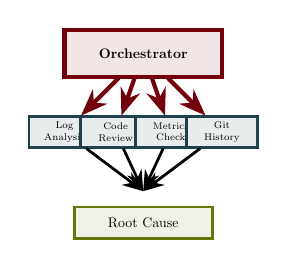
\begin{tikzpicture}[scale=0.5, transform shape]
    \node[orchestrator, minimum width=4cm] (orch) at (0,4) {Orchestrator};

    \node[task, font=\scriptsize] (t1) at (-2,2) {Log\\Analysis};
    \node[task, font=\scriptsize] (t2) at (-0.7,2) {Code\\Review};
    \node[task, font=\scriptsize] (t3) at (0.7,2) {Metrics\\Check};
    \node[task, font=\scriptsize] (t4) at (2,2) {Git\\History};

    \draw[thickarrow] (orch) -- (t1);
    \draw[thickarrow] (orch) -- (t2);
    \draw[thickarrow] (orch) -- (t3);
    \draw[thickarrow] (orch) -- (t4);

    \draw[arrow] (t1) -- (0,0.5);
    \draw[arrow] (t2) -- (0,0.5);
    \draw[arrow] (t3) -- (0,0.5);
    \draw[arrow] (t4) -- (0,0.5);

    \node[result, minimum width=3.5cm] (root) at (0,-0.3) {Root Cause};
\end{tikzpicture}
\end{center}
\end{column}
\begin{column}{0.5\textwidth}
\begin{block}{Findings Converge}
\begin{itemize}
    \item Logs: Memory allocation failure
    \item Code: No streaming, full load
    \item Metrics: Memory 100\% at crash
    \item Git: Removed streaming code
\end{itemize}
\end{block}

\begin{exampleblock}{Root Cause}
Optimization removed streaming $+$ new dependency = OOM on large payloads
\end{exampleblock}

\textbf{Time:} 10 min vs 2 hours (90\% saved)
\end{column}
\end{columns}
\end{frame}

% ============================================================
% SECTION 7: Best Practices
% ============================================================
\section{Best Practices}

% ------------------------------------------------------------
% Slide 29: Design Principles
% ------------------------------------------------------------
\begin{frame}{Design Principles for Two-Layer Systems}
\begin{columns}[T]
\begin{column}{0.48\textwidth}
\begin{block}{Orchestrator Best Practices}
\begin{enumerate}
    \item \textbf{Plan thoroughly}\\
          Identify parallelizable work early
    \item \textbf{Provide context efficiently}\\
          Only what workers need
    \item \textbf{Write clear instructions}\\
          Specific, measurable criteria
    \item \textbf{Handle failures gracefully}\\
          Expect some workers to fail
\end{enumerate}
\end{block}
\end{column}
\begin{column}{0.48\textwidth}
\begin{block}{Worker Best Practices}
\begin{enumerate}
    \item \textbf{Understand scope}\\
          Stay focused on assigned task
    \item \textbf{Use provided context}\\
          Do not expand beyond it
    \item \textbf{Validate output}\\
          Check against criteria
    \item \textbf{Report clearly}\\
          Structured, concise findings
\end{enumerate}
\end{block}
\end{column}
\end{columns}

\vspace{0.3cm}
\begin{center}
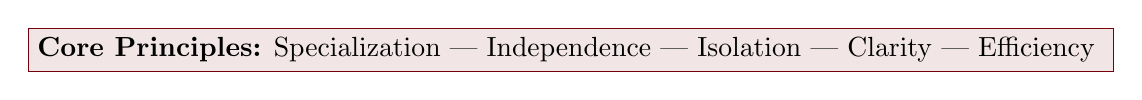
\begin{tikzpicture}
    \node[fill=UofSCGarnet!10, draw=UofSCGarnet, minimum width=11cm, align=center] {
        \textbf{Core Principles:} Specialization | Independence | Isolation | Clarity | Efficiency
    };
\end{tikzpicture}
\end{center}
\end{frame}

% ------------------------------------------------------------
% Slide 30: Common Pitfalls
% ------------------------------------------------------------
\begin{frame}{Common Pitfalls and How to Avoid Them}
\begin{columns}[T]
\begin{column}{0.48\textwidth}
\begin{alertblock}{Over-Parallelization}
\textbf{Problem:} Spawn 100 tasks for simple job\\
\textbf{Fix:} Use only for 3+ substantial tasks
\end{alertblock}

\begin{alertblock}{Poor Task Definition}
\textbf{Problem:} ``Do something smart''\\
\textbf{Fix:} Specific instructions with criteria
\end{alertblock}

\begin{alertblock}{Context Bloat}
\textbf{Problem:} Entire codebase to each worker\\
\textbf{Fix:} Only relevant files within 200K
\end{alertblock}
\end{column}
\begin{column}{0.48\textwidth}
\begin{alertblock}{Unhandled Dependencies}
\textbf{Problem:} Parallel tasks that depend on each other\\
\textbf{Fix:} Identify deps early, serialize when needed
\end{alertblock}

\begin{alertblock}{Ignoring Failures}
\textbf{Problem:} No fallback when workers fail\\
\textbf{Fix:} Use partial results, retry, or redesign
\end{alertblock}

\begin{alertblock}{Too Many Tasks}
\textbf{Problem:} Spawn 50 tasks at once\\
\textbf{Fix:} Batch into groups of $\leq$10
\end{alertblock}
\end{column}
\end{columns}
\end{frame}

% ------------------------------------------------------------
% Slide 31: Metrics
% ------------------------------------------------------------
\begin{frame}{Measuring Success: Key Metrics}
\begin{center}
\begin{tabular}{>{\bfseries}l p{5cm} p{3cm}}
\toprule
Metric & Description & Target \\
\midrule
Time Efficiency & Sequential / Parallel time & 3--8x speedup \\
\addlinespace
Quality & Result improvement vs single agent & 20--40\% better \\
\addlinespace
Cost & Tokens used per work unit & $\leq$ sequential \\
\addlinespace
Reliability & Worker success rate & $>$90\% \\
\addlinespace
Scalability & Time vs problem size & Sublinear \\
\bottomrule
\end{tabular}
\end{center}

\vspace{0.3cm}
\begin{block}{Decision Framework}
\begin{itemize}
    \item Speedup $>$ 2x? Continue with two-layer
    \item Speedup $<$ 1.5x? Reconsider design
    \item Failure $>$ 10\%? Task definitions need work
\end{itemize}
\end{block}
\end{frame}

% ============================================================
% SECTION 8: Summary
% ============================================================
\section{Summary}

% ------------------------------------------------------------
% Slide 32: Summary
% ------------------------------------------------------------
\begin{frame}{Two-Layer Agent Architecture: Summary}
\begin{columns}[T]
\begin{column}{0.48\textwidth}
\begin{block}{Core Concept}
Orchestrator-Worker Pattern
\begin{itemize}
    \item Orchestrator: Plans, delegates, decides
    \item Workers: Execute, report, specialize
    \item Together: Solve complex problems fast
\end{itemize}
\end{block}

\begin{exampleblock}{Key Benefits}
\begin{itemize}
    \item Parallelization (3--8x speedup)
    \item Specialization (20--40\% quality)
    \item Scalability (easy to add workers)
    \item Resilience (isolated failures)
\end{itemize}
\end{exampleblock}
\end{column}
\begin{column}{0.48\textwidth}
\begin{block}{When to Use}
\begin{itemize}
    \item Complex, decomposable work
    \item 3+ independent tasks
    \item Total work $>$ 2--3 hours
    \item Parallelization beneficial
\end{itemize}
\end{block}

\begin{block}{Claude Code Implementation}
\begin{itemize}
    \item Main agent = Orchestrator
    \item \texttt{task: "..."} = Worker spawn
    \item Up to 10 concurrent
    \item $\sim$200K tokens each
\end{itemize}
\end{block}
\end{column}
\end{columns}

\vspace{0.3cm}
\begin{center}

\begin{tikzpicture}
    \node[fill=UofSCGarnet, text=UofSCWhite, minimum width=12cm, align=center, font=\bfseries] {
        Key Insight: Think like a manager, not a worker. Plan and delegate.
    };
\end{tikzpicture}
\end{center}
\end{frame}

% ------------------------------------------------------------
% Final Slide: Questions
% ------------------------------------------------------------
\begin{frame}[plain]
\begin{center}
\vspace{2cm}
{\Huge\bfseries\textcolor{UofSCGarnet}{Questions?}}

\vspace{1cm}

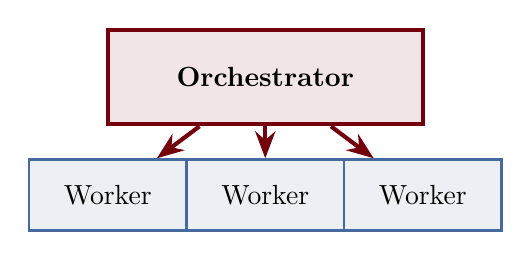
\begin{tikzpicture}
    \node[orchestrator, minimum width=4cm] (orch) at (0,1) {Orchestrator};
    \node[worker] (w1) at (-2,-0.5) {Worker};
    \node[worker] (w2) at (0,-0.5) {Worker};
    \node[worker] (w3) at (2,-0.5) {Worker};

    \draw[thickarrow] (orch) -- (w1);
    \draw[thickarrow] (orch) -- (w2);
    \draw[thickarrow] (orch) -- (w3);
\end{tikzpicture}

\vspace{1cm}
{\large Two-Layer Agent Architecture}\\
{\small Teaching Agentic Coding Tools}
\end{center}
\end{frame}

\end{document}
